\chapter{ Designing New Recommender Bots }
\label{chap-bot}

Based on findings from the previous chapter, automated recommendations containing \framework are preferred by software engineers and influence their development practices. The studies presented analyzed \framework through the \suggs feature, and show that developers are more likely to adopt tool recommendations from systems incorporating this framework~\cite{RecommendationStyles} in addition to showing the suggestions made through this feature are effective for making and receiving code improvement recommendations and improving the coding activity and collaboration of peers on pull requests~\cite{SuggUnderstanding}. However, the thesis of this dissertation argues that \framework is able to improve code quality and developer productivity. To investigate this claim, I developed a new system, \tooltwo, that incorporates each of the design principles from this conceptual framework and present an evaluation of this system exploring its impact on the quality and productivity of programmers' work. Study materials for this work are available in Appendix~\ref{app-bot}.

\section{Study Rationale}

Undergraduate Computer Science courses are constantly evolving to handle the significant increase of students~\cite{Kay98Intro}. For example, educators have turned to many different automated tools to complete instructional tasks such as grading assignments and generating feedback on student code~\cite{Wilcox2015Automation}. However, studies show that despite increasing enrollment and the advantages of automated systems in the classroom, the dropout out rate in Computer Science, especially among first and second year students, is also growing. Beaubouef and colleagues suggest a primary reason for high attrition in these courses is poor behavior, such as ignoring software development processes, on programming assignments~\cite{beaubouef2005high}. To further explore the impact of \framework on improving developer behavior, this work seeks to apply this framework to make recommendations to students on programming projects. Decision-making is vital in software engineering~\cite{WooDecision}, however students frequently make poor choices and adopt bad programming behaviors when writing code for projects~\cite{Edwards09Behaviors}. Furthermore, these behaviors persist among professional software engineers who also often underestimate the time and effort required to complete development tasks~\cite{Boehm1984SEEcon}, leading to further problems such as inadequately tested software~\cite{Whittaker00Testing} and insufficient documentation~\cite{Briand03Documentation}.

\subsection{Research Questions}

To examine the impact of digital nudges for improving the behavior of students on programming assignments, we seek to answer the following research questions:

\begin{itemize}[topsep=0pt,itemsep=-1ex,partopsep=1ex,parsep=1ex]
  \item[\textbf{RQ1}] How do nudges impact the quality of student projects?
  \item[\textbf{RQ2}] How do nudges influence student productivity?
\end{itemize}

To answer these questions, I performed a study implementing \tooltwo, a system that utilizes \framework to recommend beneficial software engineering behaviors to students, on projects for an introductory undergraduate programming course. The effectiveness of this system was evaluated by examining the code quality of projects and the productivity of students. Our results suggest automated nudges from \framework improved performance, increased coding activity, and prevented procrastination on assignments. The contributions of this research include \tooltwo, a novel bot for recommend software engineering practices to students on coding projects, and an evaluation of \framework this system on improving the software engineering behaviors of student programmers.

\section{\tooltwo: Implementing \FrameWork}

To analyze automated approaches for improving programmer behavior, this work posits \tooltwo. The \tooltwo system nudges students to improve their behavior on programming assignments by automatically generating and updating issues on project GitHub repositories. This bot, presented in Figure~\ref{fig:class-bot}, utilizes GitHub issues because they allow developers to manage bugs, suggest enhancements, and provide feedback on repositories~\cite{Issues}. Furthermore, prior work suggests the GitHub issue tracker is useful for making recommendations to developers~\cite{bissyande2013issues}. 

To improve student programming behaviors, \tooltwo encouraged them to follow the \textit{software development process}, or set of activities necessary to develop and maintain software applications. This procedure includes activities related to the \textit{Requirements}, \textit{Design}, \textit{Implementation}, \textit{Testing}, and \textit{Deployment} of software. Prior work suggests students failing to follow the software development process leads to high attrition in undergraduate Computer Science courses~\cite{beaubouef2005high}. The generated issues from \tooltwo on student repositories contained sections for each software development process phase. For example, the \includegraphics[height=1em]{Chapter-6/images/rq.png} icon in Figure~\ref{fig:class-bot} represents the Requirements phase and activities related to understanding project guidelines, such as adding a description in the README. In each section, this system outlined rubric items for the assignment relevant to each phase. 

Automated issues from \tooltwo fit the definition of a nudge because they do not provide incentives to students for completing tasks nor prevent students from avoiding items. This system was evaluated against a baseline approach of using an online rubric to illustrate project requirements and the software phases.\footnote{An example of the online rubric is available here: \url{https://pages.github.ncsu.edu/engr-csc116-staff/2020-summer/projects/project6/rubric}} To improve the programming behaviors of undergraduate Computer Science students, \tooltwo was designed using \framework: \textit{Actionability}, \textit{Feedback}, and \textit{Locality}~\cite{Sorry2}. Below, we explain how \tooltwo incorporates each principle to improve student adherence to software engineering process phases.

\subsection*{Actionability}

Actionability involves automating tasks to encourage the adoption of developer behaviors and reducing user effort. \tooltwo incorporated this principle by programmatically analyzing project repositories to determine if students complete certain development process tasks according to the rubric. If the tool observes an item was accomplished based on recent commits to the project, then \tooltwo automatically updated the issue to indicate the task was completed. For example, the system would automatically run the unit tests for the code to determine if a project's unit tests were passing the system or validate a .gitignore file was pushed to the repository to verify the configuration file was added. Alternatively, the baseline approach was not actionable as the online rubric required students to manually seek information and compare their development progress to the assignment requirements outlined on the website.

\subsection*{Feedback}

Feedback consists of providing clear and coherent information to users in automated notifications. \tooltwo implements a simple feedback mechanism to present information to students on their adherence to software engineering processes. The system displayed a red x (\includegraphics[height=1em]{Chapter-6/images/x.png}) if the assignment requirements for a project task were not completed. When the bot detected a task was completed, it automatically updated the feedback icon next to the rubric item listed in the GitHub issue to be a green check mark (\includegraphics[height=1em]{Chapter-6/images/check.png}). For instance, in the Deployment phase of the \tooltwo example in Figure~\ref{fig:class-bot}, the project repository does contain a .gitignore file but the source code does not compile. However, with the baseline approach students were not provided with any feedback on their project and were forced to determine if project expectations are met on their own.


\subsection*{Locality}

Locality refers to the setting of automated recommendations, specifically when and where interventions are displayed to users during the development processes. To promote \textit{spatial locality}, \tooltwo recommendations were implemented as GitHub issues located on the project repository within the issue tracker. To support \textit{temporal locality}, the system automatically analyzed repositories daily to provide regular updates to the \tooltwo software development processes issues based on students' recent commits and code contributions to their project. However, the baseline approach does not incorporate temporal or spatial locality in that it forced students to search for information at a separate location from their repository on the course website and in ad hoc manner without any specified timing.

\begin{figure}[htbp]
\centering
	\includegraphics[width=0.65\textwidth]{Chapter-6/images/class-bot1162.png}
	\caption{Example \tooltwo recommendation}	
	\label{fig:class-bot} 
\end{figure}

\section{Methodology}

To explore the impact of digital nudges on code quality and developer productivity, we implemented a mixed methods study to analyze \framework on student behavior for projects in a university-level introductory Java programming course.

\subsection{Data Collection}

\subsubsection{Participants} 

Participants were undergraduate students enrolled in an introductory Java programming class. The students were from different majors, demographics, and levels of programming experience. For consistency in our data, students who enrolled and then eventually dropped the class were eliminated from this evaluation. Overall, we observed the behavior of 35 out of the initial 42 registered students. The participants were aware of the five phases used to define the software development process: \textit{Requirements}, \textit{Design}, \textit{Implementation}, \textit{Test}, and \textit{Deployment}, as presented to students in the course curriculum.

\subsubsection{Projects}

To analyze \framework in \tooltwo, we observed and nudged developer behaviors to students on introductory Java programming projects. For the semester the course consisted of seven programming assignments, six projects and a final comprehensive exercise. Projects 3-5 made up the control group for this experiment to avoid the beginning assignments (Projects 1 and 2). \tooltwo was introduced to students on the final two assignments of the course, Project 6 and the Comprehensive Exercise, to examine its impact on the quality of projects and productivity of students. All coding projects for the were hosted and submitted on GitHub repositories. In total, we analyzed a total of 151 projects from students.

\subsubsection{Developer Behavior}

To improve the decision-making of programmers, the developer behavior \tooltwo focused on encouraged students to follow the software engineering process. Prior work by Beaubouef and colleagues suggests students' failure to adhere to development processes factors into the high attrition rate and failure rate in early programming courses. For example, they note the following about typical student programming methods:

\begin{quote}
``\textit{This [students' estimated time to complete projects] minimally includes the processes of analysis, design, coding, testing, and documentation. Software projects developed by professionals are notoriously behind schedule in the real world. It should come as no surprise that software developed (programs written) by students will tend to be even more behind schedule.} 

\textit{Unsuccessful students often want to skip analysis and design and begin typing in code immediately. Documentation is an afterthought at best, and little or  no testing is performed. Because the student planned to attack the assignment in this manner from the beginning, he will often wait until the last minute to begin and work until its done or time runs out. These students set themselves up for frustration, unnecessary rework, and failure.}''~\citep[p.~105]{beaubouef2005high}
\end{quote}

We define the software development process as \textit{Requirements}, \textit{Design}, \textit{Implementation}, \textit{Test}, and \textit{Deployment}. These phases were derived from the course materials and introduced to students during a lecture before \tooltwo was introduced on projects for this study. Our goal is to use \framework to encourage students to complete all of the software process phases for their projects. Each project contained a \tooltwo issue with sections for each phase listing the relevant tasks. Specific items listed differed based on the project requirements, however in general: Requirements (\texttt{Rq}) focused on activities to understand assignment specifications; Design (\texttt{Ds}) referred to the organization of code and project structure; Implementation (\texttt{Im}) centered on the development of the code; Testing concentrated on actions to develop unit tests (\texttt{Ut}) and functional test cases (\texttt{St}); and Deployment (\texttt{Dp}) concentrated on actions to verify the project and repository were ready for submission. When students completed a specific task, \tooltwo would automatically update the issue to indicate the item was completed.

\subsection{Determining the effectiveness of \tooltwo}

To examine the impact of \tooltwo on student behavior, we mined GitHub repositories to observe metrics measuring its impact on the quality of students' work and the productivity of their project development.

\subsubsection{Quality}

To answer RQ1, we evaluated the quality of student projects by examining their overall \textit{grade} on the assignment in addition to the number of \textit{points deducted} from the project due to students not adhering to requirements for the assignment.

\paragraph*{Grade}

For coding projects, the assignment grade indicates the overall quality of the project. Research suggests poor project management skills~\cite{beaubouef2005high} and ineffective behaviors~\cite{Edwards09Behaviors} result in low grades for students on programming assignments. Similarly, research shows the behavior and \textit{software process maturity} impacts the quality of programs for professional software engineering teams~\cite{Clark97theeffects}. Within the course analyzed for this study, project grades were determined by real-world software engineering quality metrics, such as passing unit tests and functional test cases, Checkstyle\footnote{\url{https://checkstyle.sourceforge.io/}} static analysis tool warnings, and correct project structure. To determine how well \tooltwo supports students in software process decisions, we analyzed projects with and without nudges from this system to determine how this approach impacted the overall grade of coding assignments as a method to determine the project quality.

\paragraph*{Deductions}

Another determinant of project quality is the number of points deducted on student programs. In education, grading penalties are commonly used to encourage students to perform better on assignments~\cite{Reeves2017SpecialTW}. Students who failed to meet certain requirements designated for the project had additional points subtracted from their overall grade. For example, submitting an assignment within 24 hours after the deadline resulted in a -10\% late penalty. In this study, we analyzed projects with and without notifications from \tooltwo to determine if \framework improves student behavior and project quality by minimizing the number of points deducted from programs.

\subsubsection{Productivity}

To answer RQ2, this study examines if nudges impact the productivity of students working on programming assignments.
We measured productivity by observing several different metrics mined from GitHub repositories, including the total \textit{number of commits}, \textit{code churn}, the amount of time until the \textit{first commit}, and the timing
between the \textit{last commit} and the assignment deadline.

\paragraph*{Commits}

GitHub commits are used to record specific changes
made to the project files.\footnote{\url{https://docs.github.com/en/desktop/contributing-and-collaborating-using-github-desktop/committing-and-reviewing-changes-to-your-project\#about-commits}} Prior work in Computer Science education explores analyzing repository commits on version control systems to encourage students to make more frequent contributions to projects~\cite{Singer12Race} and predict student performance~\cite{sprint2019mining}. In industry, commits have been used to measure contributions from programmers as well as the prolificacy of developers on GitHub~\cite{Vasilescu2016Multitask}. To discover if nudging students enhances productivity, we compared the total number of commits submitted by students to their project repositories with and without \tooltwo notifications.

\paragraph*{Code Churn}

To determine the impact of automated nudges from
our system on the activity of students, we also analyzed the code churn of commits made to repositories on assignments with and without updates from \tooltwo. Prior work in software engineering suggests code churn is a useful metric measuring effort and the impact of code changes~\cite{Munson98Churn}, predicting the defect density in software~\cite{nagappan2005DefectDensity}, and analyzing GitHub contributions in the pull-based software development model~\cite{gousios2014dataset}. In this evaluation, code churn was measured by summing the number of lines added, deleted, or modified for each commit made by students to their project repository.

\paragraph*{First Commit} To further investigate the impact of \tooltwo on the productivity of students, we analyzed the timing of commits. We examined the timing of the first commit on repositories to indicate when students began development on their project. Prior work by Edwards et al. shows that students who start working on assignments earlier receive significantly higher grades on projects, while students who start later often perform worse~\cite{Edwards09Behaviors}. To calculate the first commit time, we measured the amount of time between the creation and designation of project repositories to students after the assignment was announced in class until the first commit was made on the repository. We compare the timing of the first commit to projects with and without issues from \tooltwo to determine if the automated feedback provided from this system encourages students to start earlier and prevents procrastination on programming assignments.

\paragraph*{Last Commit}

We also analyzed the timing of the last commit on repositories to signify students completing work on their project. Edwards also found the time of last submission on a student programming project also significantly impacts their performance~\cite{Edwards09Behaviors}. To help students be more productive and discourage late submissions, we aim to user \tooltwo to nudge students to complete software development tasks. To further explore the impact of \framework on productivity, we calculated the amount of time between the last commit on a project repository and the project deadline to measure the last commit time. \\

Overall, we use these quality and productivity metrics to investigate the impact of bots incorporating \framework on the software engineering behaviors of students working on programming projects.

\subsubsection{Survey}
 
Additionally, at the end of the semester we sent students a survey to collect qualitative data on their experience with
\tooltwo on their repositories. The survey contained a 5-point Likert scale question asking students about the
usefulness of updates from this system and sought open-ended feedback to describe what they find useful about the automated updates against manually checking the website and to provide any additional comments about the system. We disseminated the survey to students after the last day of class and the completion of the projects and course assignments. Out of the 35 eligible students, we received 9 responses from participants (25.7\% response rate). To analyze the survey data, Likert scale responses were aggregated to determine the usefulness of \tooltwo and we analyzed open-ended responses to derive feedback from students on improving automated bots for enhancing programmer behavior. 

\section{Results}

To examine the impact of \framework, this work analyzed the impact of notifications from \tooltwo on the behavior of students working on programming projects. The Mann-Whitney-Wilcoxon test ($\alpha$ = .05) was used to analyze the project quality and student productivity metrics for assignments with and without nudges from \tooltwo.

\subsection{RQ1: Quality}

To observe the impact of automated nudges incorporating \framework on code quality, we analyzed the grade and number of points deducted on student assignments with and without \tooltwo recommendations. The code quality results are presented in Table~\ref{tab:quality}. For grading, students received an average of 2.6 points higher on assignments with automated nudges. Additionally, we found students received significantly higher scores on projects with automated nudges ($p = 0.0097$). This demonstrates notifications from the \tooltwo system improved the overall quality of programming assignments. Additionally, while there was not a significant difference, we noticed projects without automated nudges had an average of 11 more points deducted compared to those with \tooltwo interventions.

\subsection{RQ2: Productivity}

To discover the impact of \tooltwo on development productivity, we analyzed the total commits, code churn, first commit time, and last commit time on student project repositories. Our results, presented in Table~\ref{tab:productivity}, show that projects with nudges increased development activity approximately three more commits and 897 more lines of code changed for each commit. Additionally, we found this approach improved the timing of student work by encouraging participants to begin work around six days earlier and to submit assignments 12 hours sooner.\footnote{A negative result here indicates assignments submitted late after the deadline}. Furthermore, we found that \tooltwo significantly increased the number of lines of code modified in commits (\textbf{\em code churn}, $p = 0.0348$) and significantly prevented procrastination (\textbf{\em first commit}, $p < 0.0001$). Overall, this signifies that nudges from \tooltwo improved the productivity of students working on programming assignments.


\begin{table}[tbh]
\centering
\caption{\tooltwo Quality Results}
\begin{threeparttable}
\begin{tabular}{ |l|l|r|r|c| } \hline
  \textbf{} & \textbf{Nudge?} & \textbf{Mean} & \textbf{Median} & \textbf{\textit{p-value}} \\ \hline
 \multirow{2}{*}{\textbf{Grade***}} & No & 74.29 &  87.66 & - \\
 & Yes & 76.89 & 95 &  \textbf{\em 0.0097***}  \\ \hline
 \multirow{2}{*}{\textbf{Deductions}} & No & -20.71 & -5 & - \\
 & Yes & -9.43 & 0 &  0.0672 \\ \hline
\end{tabular}
\begin{tablenotes}
% \centering
\textbf{***} denotes statistically significant results (\textit{p-value} $< 0.05$)
\end{tablenotes} 
\end{threeparttable}
\label{tab:quality}
\end{table}

\begin{table}[tbh]
\centering
\caption{\tooltwo Productivity Results}
\begin{threeparttable}
\begin{tabular}{ |l|l|r|r|c| } \hline
  \textbf{} & \textbf{Nudge?} & \textbf{Mean} & \textbf{Median} & \textbf{\textit{p-value}} \\ \hline
 \multirow{2}{*}{\textbf{Commits}} & No & 9.84 & 7 & - \\
 & Yes & 12.64 & 9 & 0.1646 \\ \hline
 \multirow{2}{*}{\textbf{Code Churn***}} & No &  205.03 & 4 & - \\
 & Yes & 1101.57 & 11 & \textbf{\em 0.0348***} \\ \hline
 \multirow{2}{*}{}\textbf{First Commit***} & No &  8.32 & 7.41 & - \\
 \textbf{(days)} & Yes & 1.99 & 5.94 & \textbf{\em $<$ 0.0001***} \\ \hline
  \multirow{2}{*}{}\textbf{Last Commit} & No &  -21.72 & -1.60 & - \\
 \textbf{(hours)} & Yes & -9.67 & -2.47 &  0.7909 \\ \hline
\end{tabular}
\begin{tablenotes}
% \centering
\textbf{***} denotes statistically significant results (\textit{p-value} $< 0.05$)
\end{tablenotes} 
\end{threeparttable}
\label{tab:productivity}
\end{table}

\subsection{Survey}

To further evaluate the \tooltwo system, we surveyed students to collect feedback on their experience with this bot on their repositories. Figure~\ref{fig:class-survey} shows Likert scale questions results on students' perceptions of the usefulness of the automated nudges. Overall, most respondents (88.9\%) found the notifications from \tooltwo at least moderately useful. Participants commented on the \tooltwo interventions on their projects noting they ``\textit{liked the class-bot updates}'' (P1) and used it to ``\textit{make sure everything was running smoothly}'' (P6). We analyzed open-ended responses and derived two themes to provide insight into improving automated tools for recommending developer behaviors to programmers.

\begin{figure}[htb]
\centering
 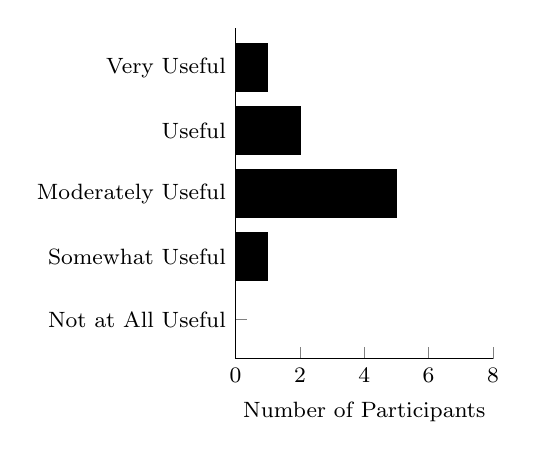
\begin{tikzpicture}
 \begin{axis}[
     xbar stacked,
     ytick=data,
     axis y line*=none,
    axis x line*=bottom,
    tick label style={font=\footnotesize},
    legend style={font=\footnotesize},
    label style={font=\footnotesize},
    xtick={0,2,4,6,8},
    width=.4\textwidth,
    bar width=6mm,
    xlabel= Number of Participants,
    yticklabels={Not at All Useful, Somewhat Useful, Moderately Useful, Useful, Very Useful},
    xmin=0,
    xmax=8,
    area legend,
    y=8mm,
    enlarge y limits={abs=0.625},
]

\addplot[fill=black] coordinates
{(0,0) (1,1) (5,2) (2,3) (1,4)};
\end{axis}  
\end{tikzpicture}
\caption{Survey Results on the Usefulness of \tooltwo}
\label{fig:class-survey}
\end{figure}


\subsubsection{Validation Frequency}

One area of improvement for the \tooltwo system is to improve how students verify their project. Even though we found students started programming assignments significantly earlier when automated issues were present, we also found that students reported waiting until the end of the development process to validate their work met the project expectations. For example, several students noted that, while they they found \tooltwo notifications useful, they ``\textit{didn't really check them until the final day}'' (P1) and ``\textit{checked it once at the end to make sure everything was correct but thats it}'' (P7). Furthermore, P7, who ranked the system the lowest as Somewhat Useful, added ``\textit{I kept track of my own progress so I did not feel the need for this}''. This problem also exists in software engineering where, while research shows validating and verifying software through out the development process improves code quality~\cite{Wallace89Verification}, professional developers often face challenges and delay validating their program meets project requirements~\cite{Garcia08Ten}. This motivates the need for automated recommendations to better integrate into development workflows by encouraging programmers to validate their code more frequently.

\subsubsection{Update Frequency}

Similarly, participants desired more frequent updates from \tooltwo. For example, students mentioned ``\textit{I liked it but would like it more
if it could be updated more often, or maybe later in the day}`` (P1) and ``\textit{the class bot didn't update frequently enough}'' (P2). Additionally, P4 thought the bot was broken due to infrequent updates and then ``\textit{did not trust it when it started to work}''. Prior work in software engineering, including the results of the \tele study, shows that untimely notifications discourage developers from adopting recommendations~\cite{viriyakattiyaporn2009challenges, Sorry}. Furthermore, researchers found presenting static analysis tool output more frequently encouraged programmers to fix more bugs~\cite{Distefano2019Facebook}. While this system incorporated temporal locality into its design by consistently updating GitHub issues, students desired even more frequent feedback and updates from the system to support them in their work. Providing frequent updates to projects can improve the integration of automated recommendations into programmers' workflows and increase the effectiveness of digital nudges for improving the adoption of developer behaviors.

\subsection{Summary}

The results from this study show that that nudges are useful for improving student programming behaviors. Specifically, we found that \tooltwo significantly improved student grades, increased the number of changes to repositories, and encouraged students to start programming earlier. Participants also reported this system was useful and provided insight
for improving automated nudges to encourage better software
engineering behaviors by better incorporating student workflows. We analyzed this feedback and present two themes based on how frequently students checked the automated notifications from \tooltwo and how often the issues were updated.

\section{Discussion}

Ultimately, this work shows incorporating \framework into automated recommendations can improve the behavior and decision-making of developers. To support this, I implemented \tooltwo as a recommender system incorporating the conceptual framework. This system was designed to include each of the choice architecture principles by generating \textit{actionable} GitHub issues with automated updates to recommend development tasks, providing straightforward and visual \textit{feedback} to track progress on projects, and presenting updates with persistent and convenient \textit{locality} on issues in the repository during development. To analyze the impact of this approach on the behavior of programmers, I developed \tooltwo to encourage student programmers to adhere to software engineering processes in their work. 

Research shows adopting software processes is a beneficial developer behavior for improving the quality of applications~\cite{Clark97theeffects}. However, Computer Science education research shows failing to adhere to software engineering processes leads to high failure and attrition in early programming courses~\cite{beaubouef2005high}. Moreover, the adoption problem for this developer behavior translates into industry, where professional software engineers also frequently fail to follow advised development practices and inappropriately allocate the time and effort for completing tasks~\cite{Boehm1984SEEcon}. By encouraging students to follow software engineering processes, we found \tooltwo improved the code quality and developer productivity of students by boosting grades, increasing code contributions, and preventing procrastination. I believe these automated nudges incorporating \framework are a step towards encouraging Computer Science students to adopt useful developer behaviors while working on programming projects, and thus improving the behavior of software engineers.


